\documentclass[a4paper, brazil]{article}
\usepackage[utf8]{inputenc}

\usepackage[cm]{fullpage}
\usepackage{pacotesLaTeX}

\author{Thales Freitas Macêdo \\ DRE: 115 162 177}
\title{LISTA 1}

\begin{document}

\maketitle

\section{Exercício 1}

\subsection{(a)}

\begin{figure}[ht]
\centering
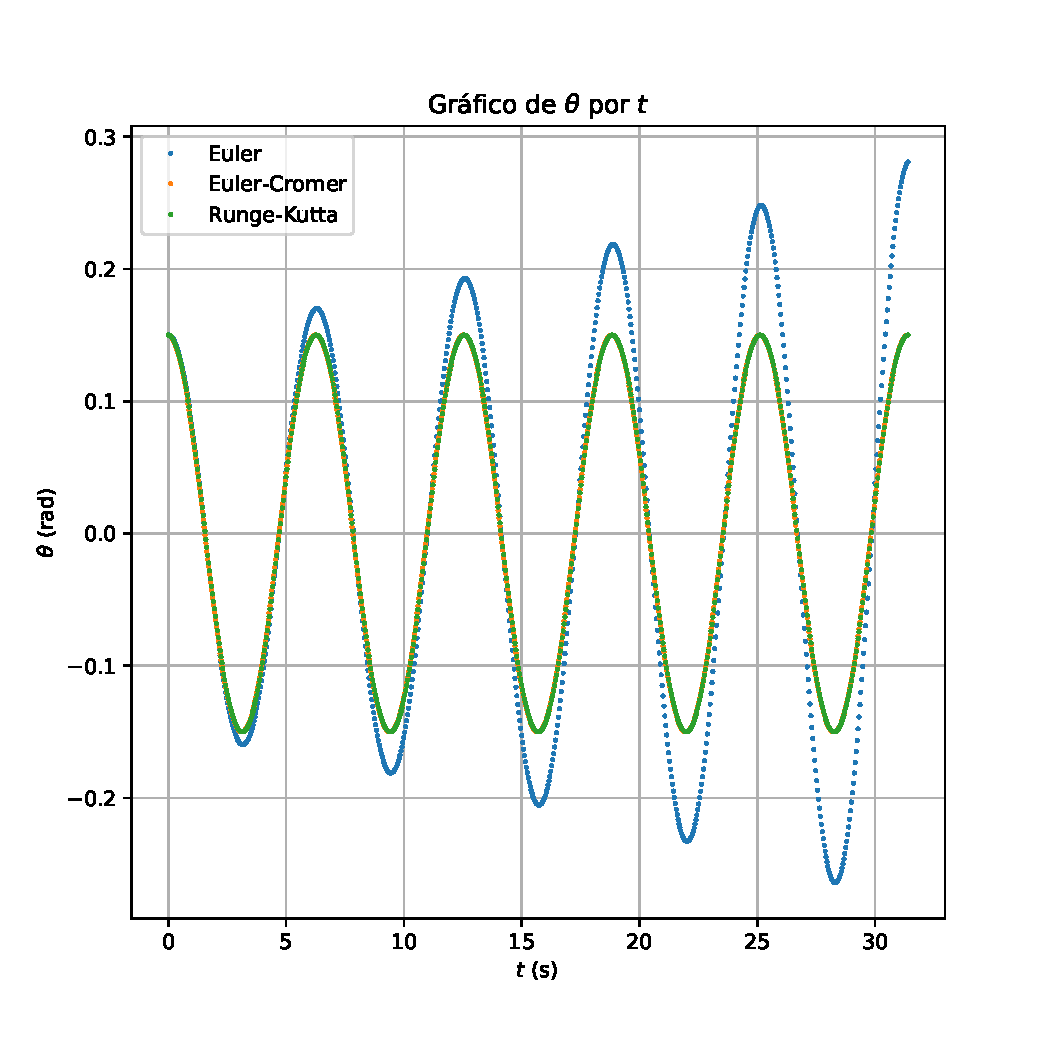
\includegraphics[width=0.7\textwidth]{fig1a.pdf}
\caption{\( \theta \) em função do tempo ao longo de 5 períodos, para os três métodos numéricos.}
\label{fig1a}
\end{figure}

A figura \ref{fig1a} mostra o gráfico de \( \theta \) em função do tempo ao longo de 5 períodos, para os métodos de Euler, Euler-Cromer e Runge-Kutta.
Esperamos que o gráfico seja de forma senoidal, com amplitude igual ao \( \theta_0 \).
O método de Euler se mostra inadequado, visto que a amplitude aumenta com o tempo.
Os métodos de Euler-Cromer e Runge-Kutta produziram o resultado esperado, e se mostram equivalentes.

\newpage
\subsection{(b)}

\begin{figure}[ht]
\centering
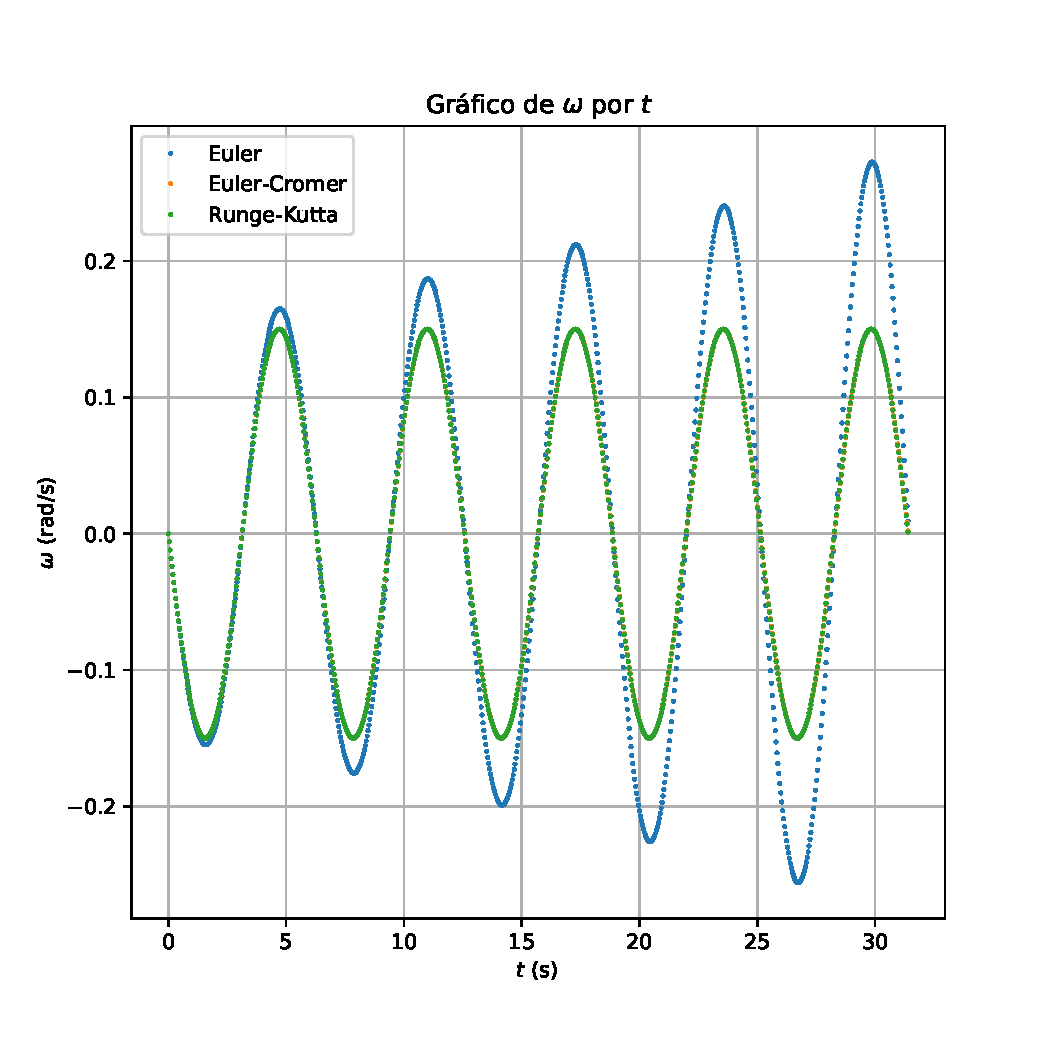
\includegraphics[width=0.7\textwidth]{fig1b.pdf}
\caption{\( \omega \) em função do tempo ao longo de 5 períodos, para os três métodos numéricos.}
\label{fig1b}
\end{figure}

A figura \ref{fig1b} mostra o gráfico de \( \omega \) em função do tempo ao longo de 5 períodos, para os métodos de Euler, Euler-Cromer e Runge-Kutta.
Esperamos que o gráfico seja de forma senoidal, com amplitude igual ao \( \Omega \theta_0 \), onde \( \Omega = \sqrt{g / l} \).
Novamente o método de Euler se mostra inadequado, visto que a amplitude aumenta com o tempo.
Os métodos de Euler-Cromer e Runge-Kutta produziram o resultado esperado, e se mostram equivalentes.

\newpage
\subsection{(c)}

\begin{figure}[ht]
\centering
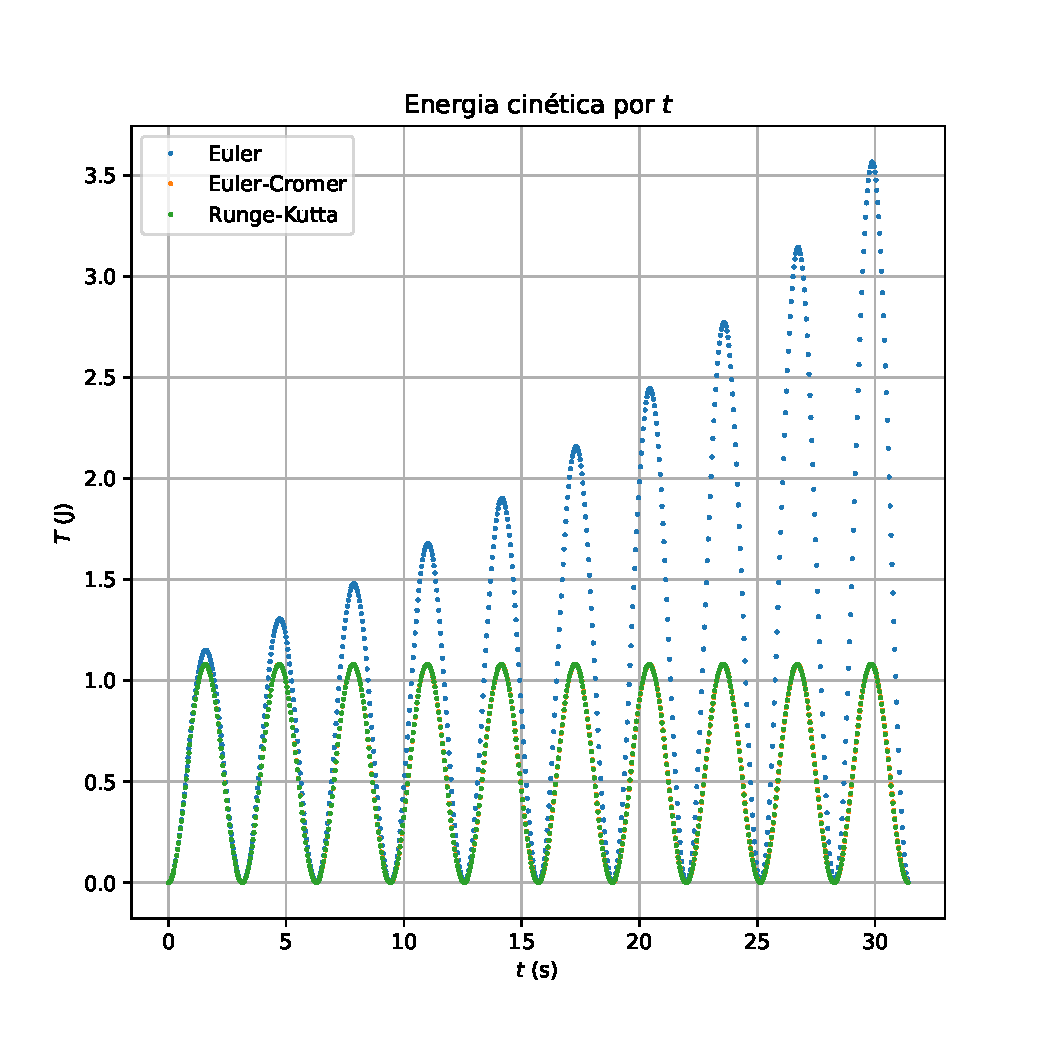
\includegraphics[width=0.4\textwidth]{fig1c1.pdf}
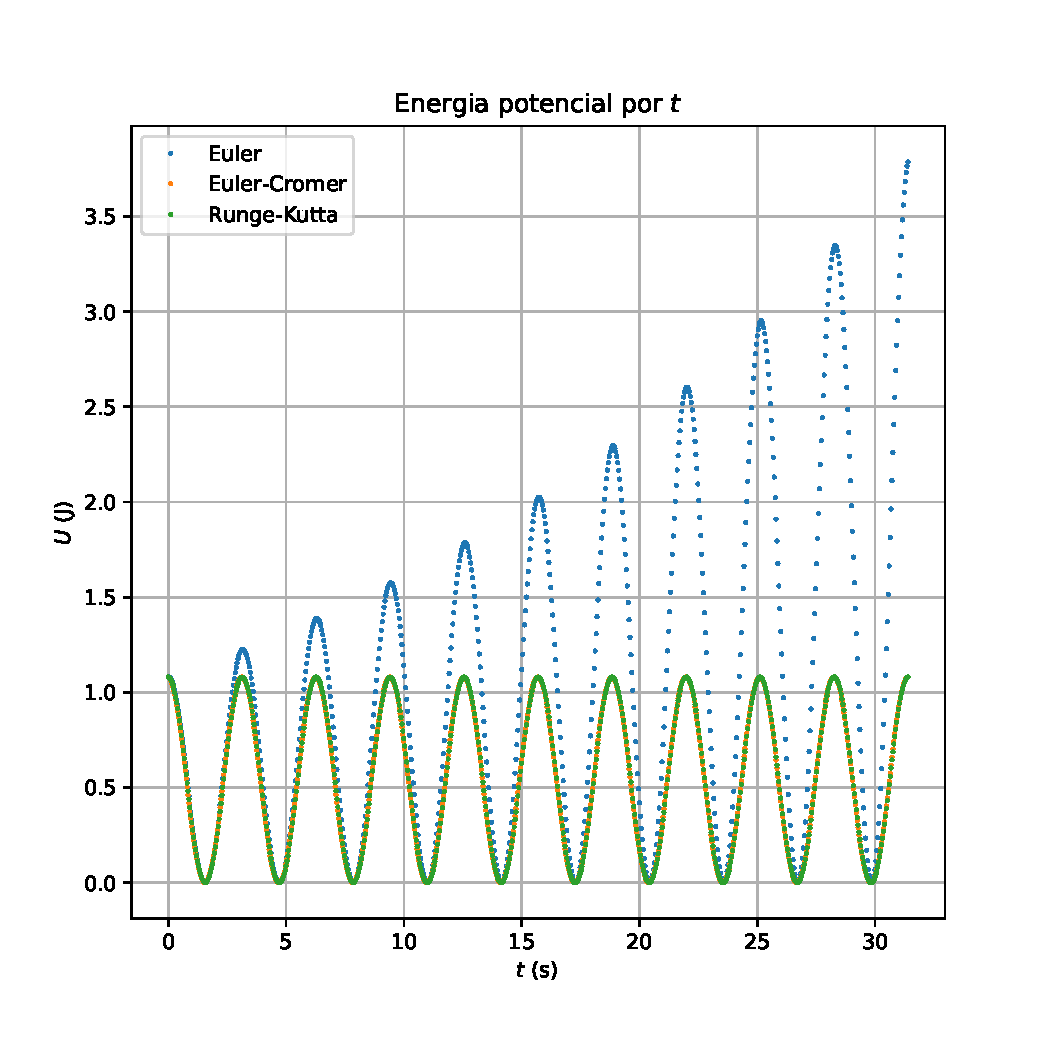
\includegraphics[width=0.4\textwidth]{fig1c2.pdf}
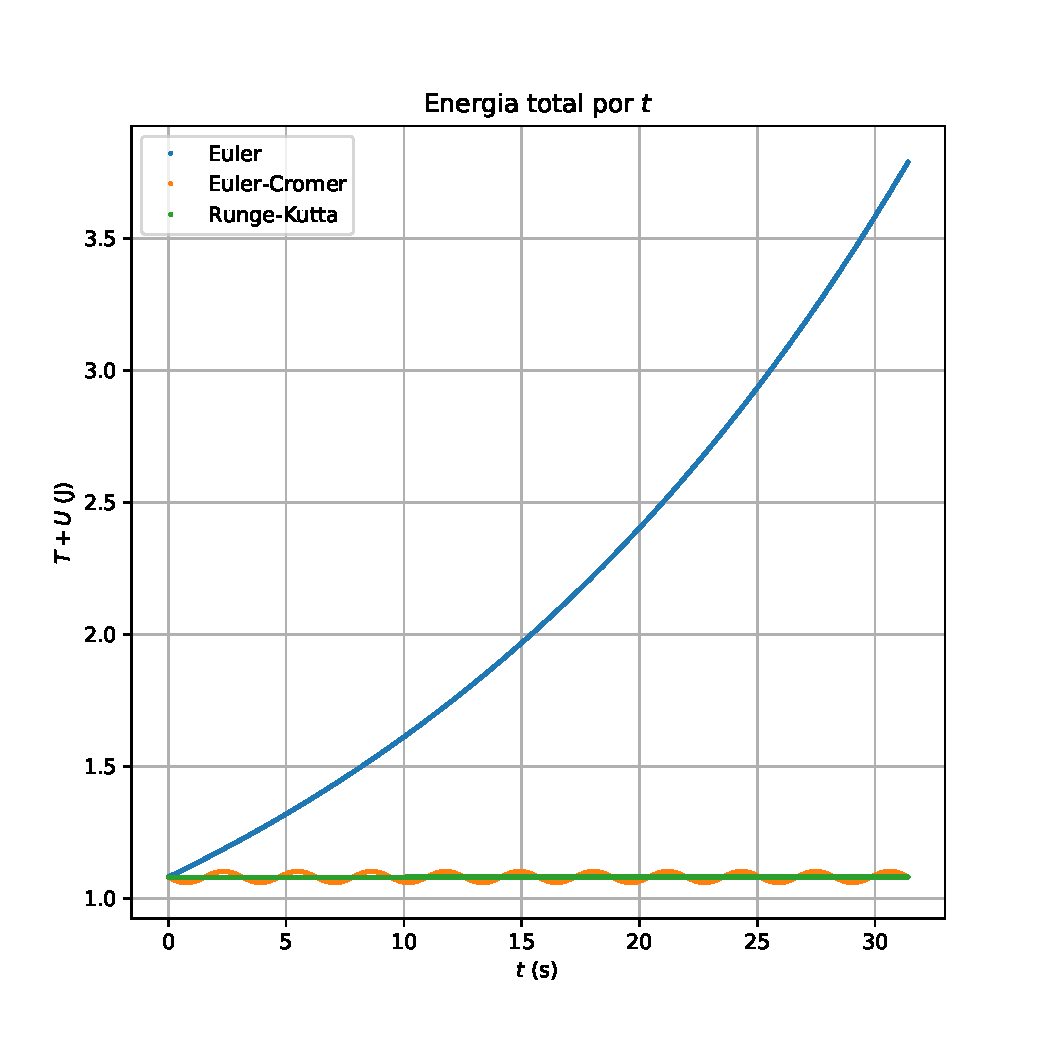
\includegraphics[width=0.4\textwidth]{fig1c3.pdf}
\caption{Energias cinética, potencial e total em função do tempo ao longo de 5 períodos, para os três métodos numéricos.}
\label{fig1c}
\end{figure}

A figura \ref{fig1c} mostra o gráfico das energias cinética, potencial e total em função do tempo ao longo de 5 períodos, para os métodos de Euler, Euler-Cromer e Runge-Kutta.
Esperamos que o gráfico das energias cinética e potencial sejam de forma senoidal, com amplitude igual à energia inicial, e que o gráfico da energia total seja constante, visto que o sistema é conservativo.
Novamente método de Euler se mostra inadequado, visto que as amplitudes das energias cinética e potencial aumentam com o tempo, e que a energia total aumenta com o tempo.
Os métodos de Euler-Cromer e Runge-Kutta produziram o resultado esperado para as energias cinética e potencial, e se mostram equivalentes nesses casos.
Para a energia total, o método de Euler-Cromer produz um gráfico senoidal com pequena amplitude em torno do valor correto, enquanto que o método de Runge-Kutta produz o resultado esperado.

\subsection{(d)}

O pior método para esse sistema físico é o método de Euler, que não conserva a energia.
O método de Euler-Cromer produz um resultado aceitável, já que conserva a energia na média.
O método de Runge-Kutta produziu o melhor resultado, já que dentro da escala do problema, a energia se manteve constante.

\newpage
\section{Exercício 2}

\subsection{(a)}

Foi escolhido o método de Runge-Kutta, com um intervalo de tempo \( \Delta t = \SI{0.01}{\second} \).
A escolha do método de Runge-Kutta se deu pelo fato de ser o mais adequado para um sistema físico similar ao usado nesse exercício, enquanto que a escolha do intervalo é devida ao balanço entre precisão e tempo de execução do programa.

\subsection{(b)}

\begin{figure}[ht]
\centering
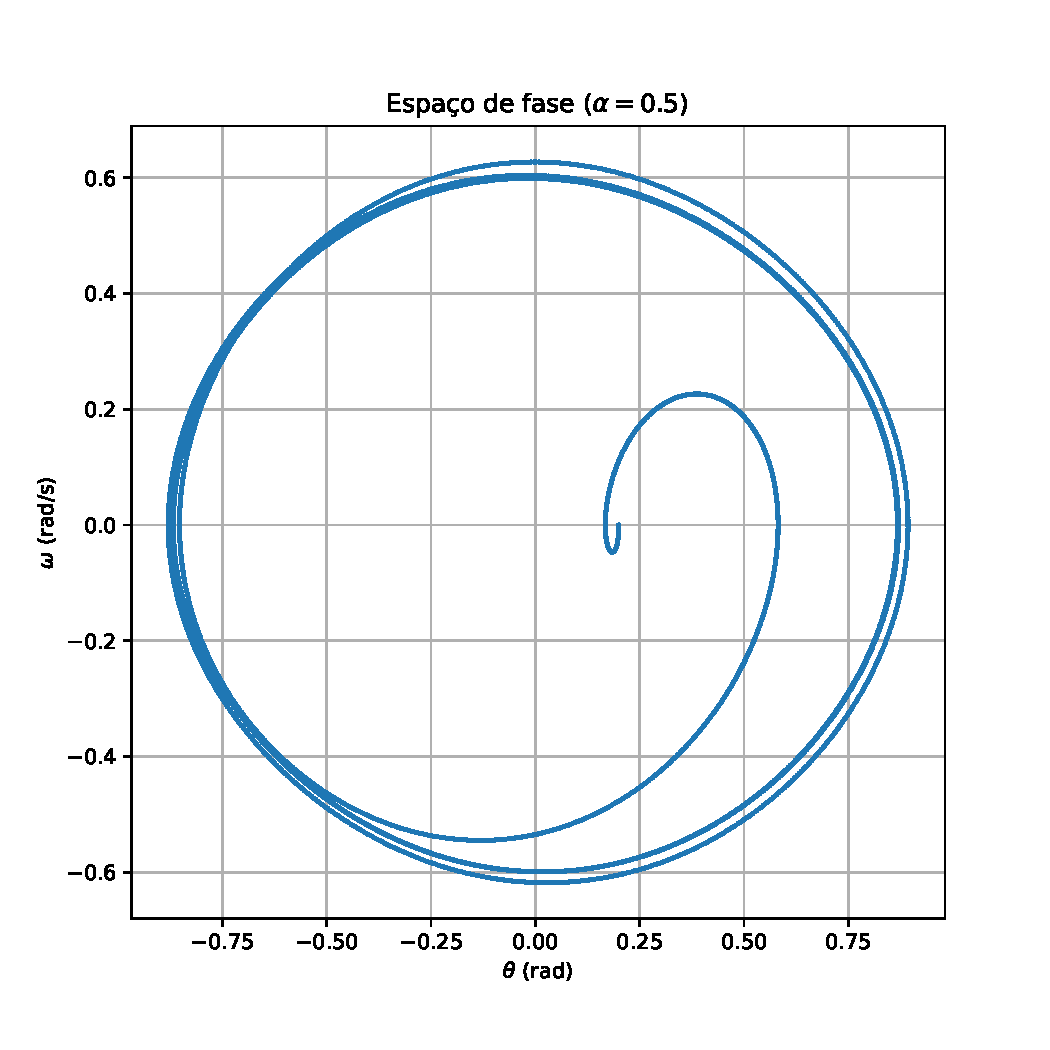
\includegraphics[width=0.4\textwidth]{fig2b1.pdf}
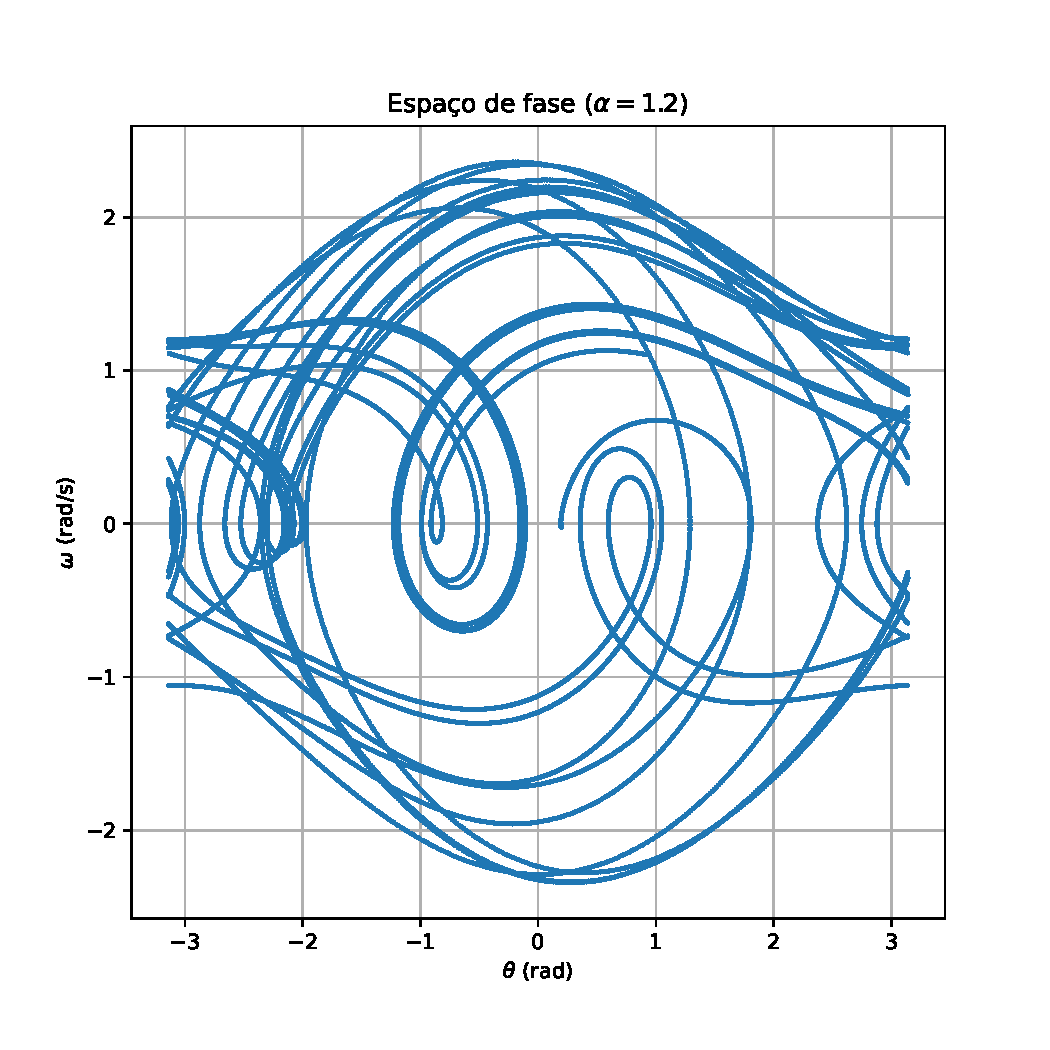
\includegraphics[width=0.4\textwidth]{fig2b2.pdf}
\caption{Trajetória no espaço de fase do pêndulo para \( \alpha = \SI{0.5}{\radian\per\second\squared} \) e \( \alpha = \SI{1.2}{\radian\per\second\squared} \).}
\label{fig2b}
\end{figure}

A figura \ref{fig2b} apresenta a trajetória no espaço de fase do pêndulo para \( \alpha = \SI{0.5}{\radian\per\second\squared} \) e \( \alpha = \SI{1.2}{\radian\per\second\squared} \).

%\newpage
\subsection{(c)}

\begin{figure}[ht]
\centering
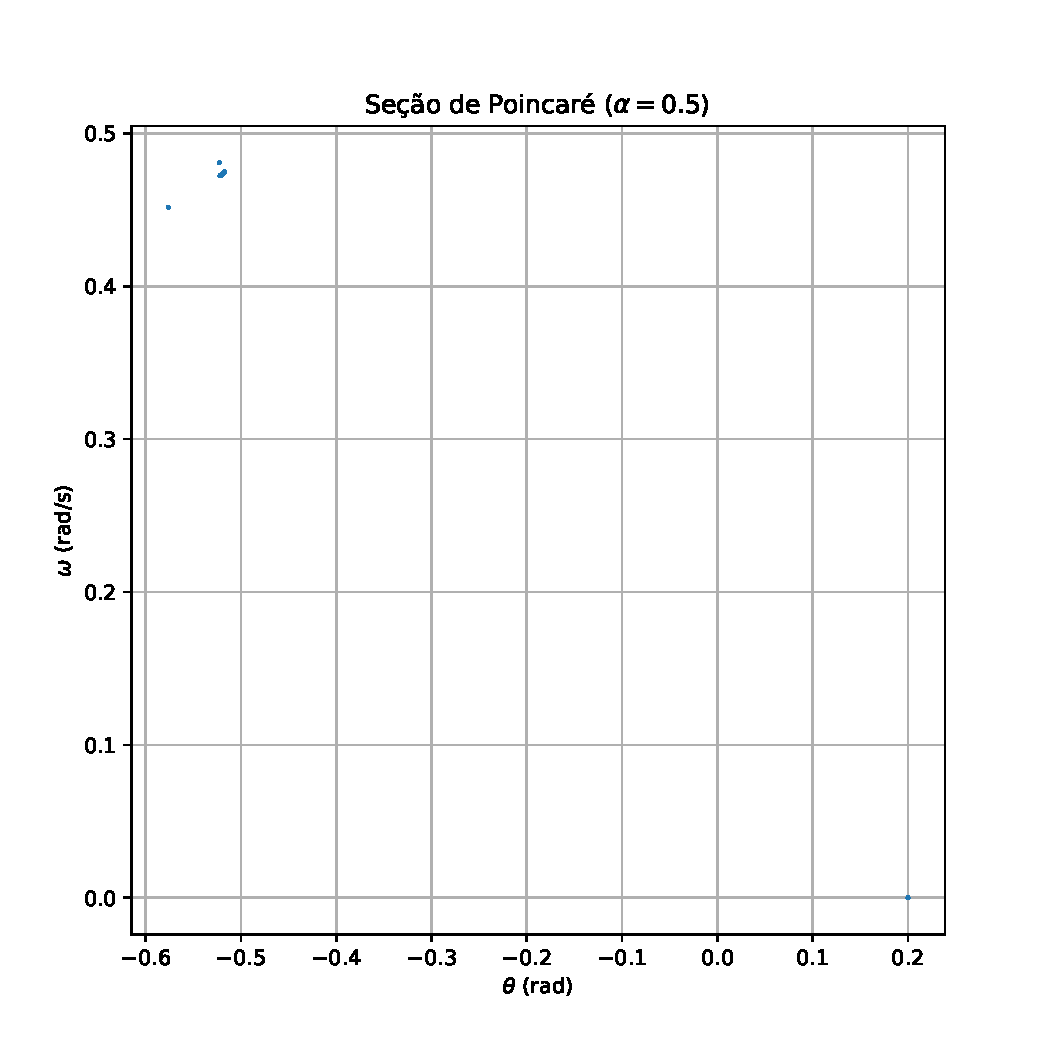
\includegraphics[width=0.4\textwidth]{fig2c1.pdf}
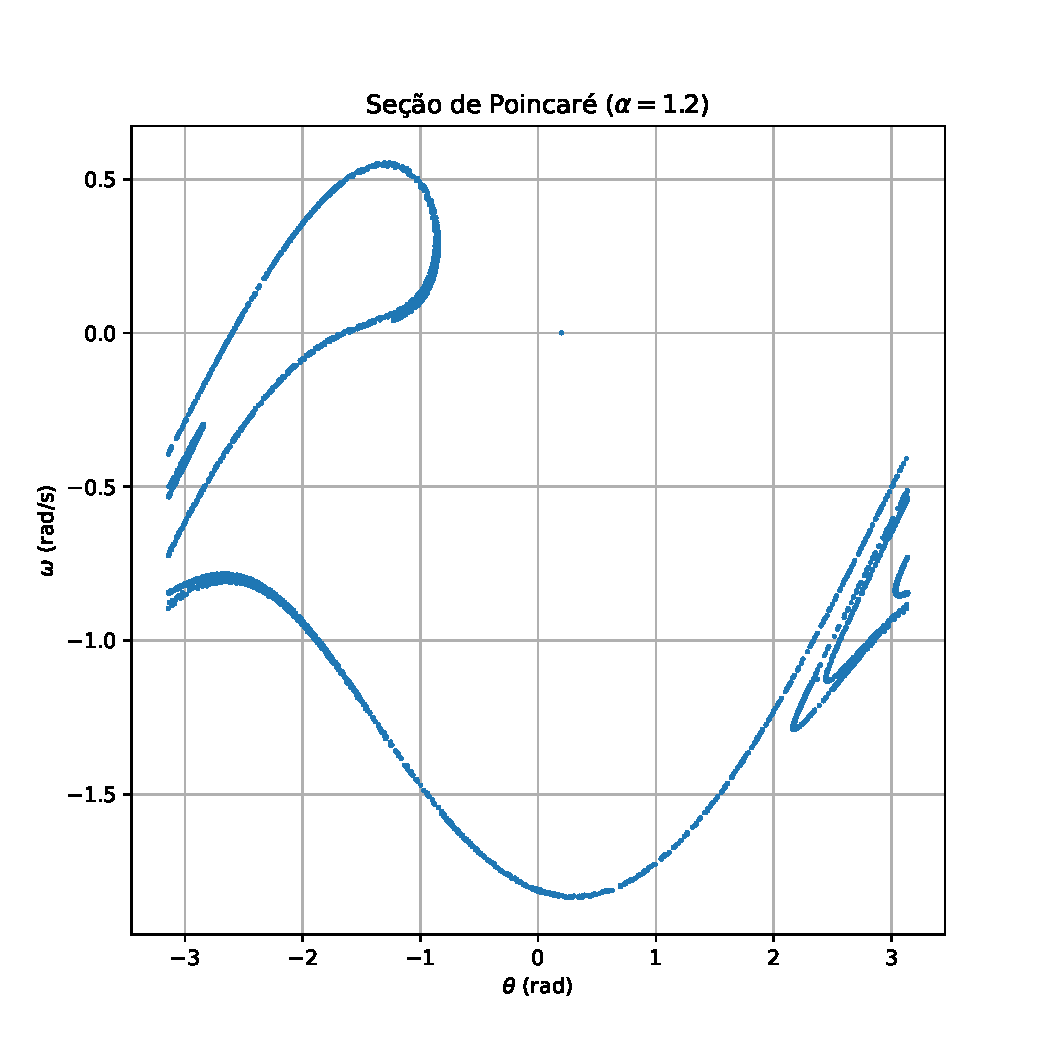
\includegraphics[width=0.4\textwidth]{fig2c2.pdf}
\caption{Seções de Poincaré do pêndulo para \( \alpha = \SI{0.5}{\radian\per\second\squared} \) e \( \alpha = \SI{1.2}{\radian\per\second\squared} \).}
\label{fig2c}
\end{figure}

A figura \ref{fig2c} apresenta a seção de Poincaré do pêndulo para \( \alpha = \SI{0.5}{\radian\per\second\squared} \) e \( \alpha = \SI{1.2}{\radian\per\second\squared} \).

\newpage
\subsection{(d)}

\begin{figure}[ht]
\centering
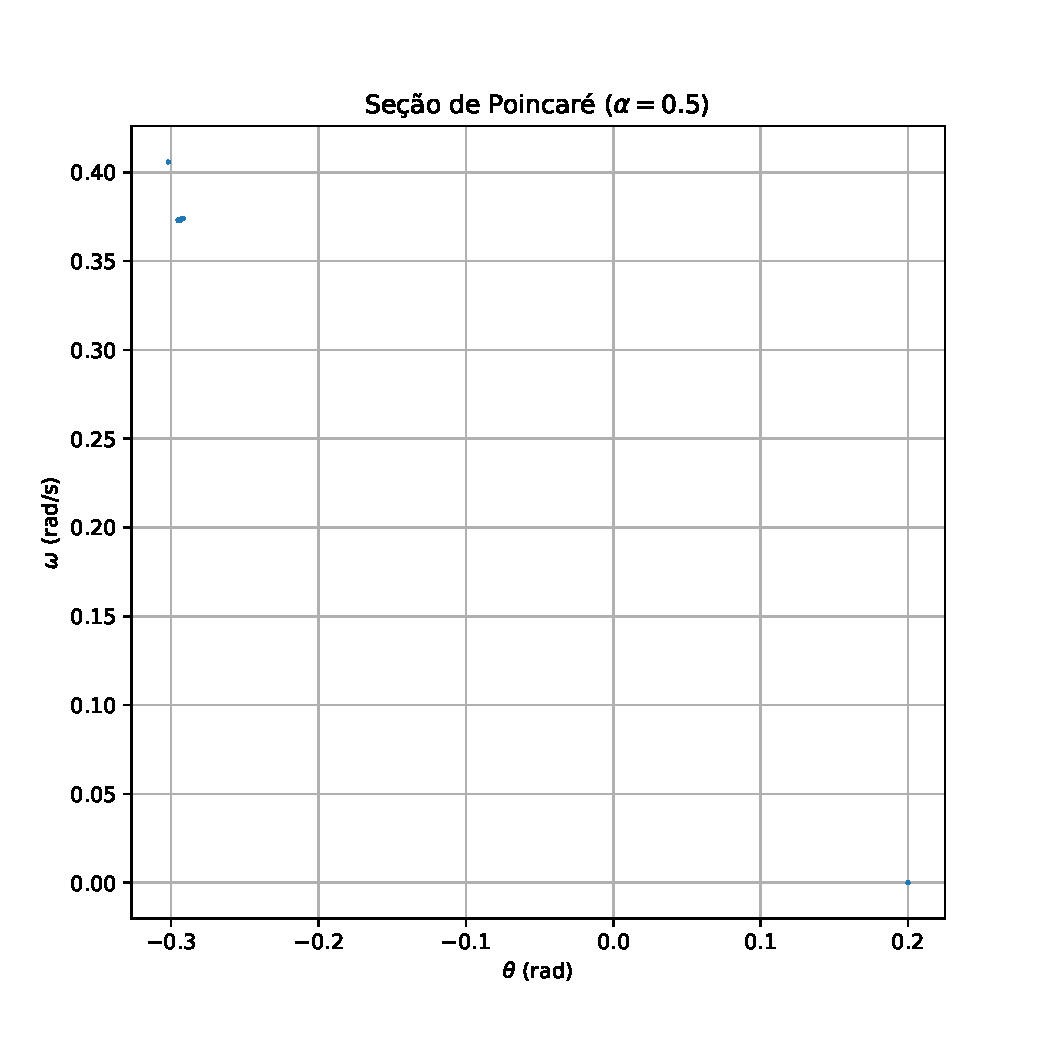
\includegraphics[width=0.4\textwidth]{fig2d1.pdf}
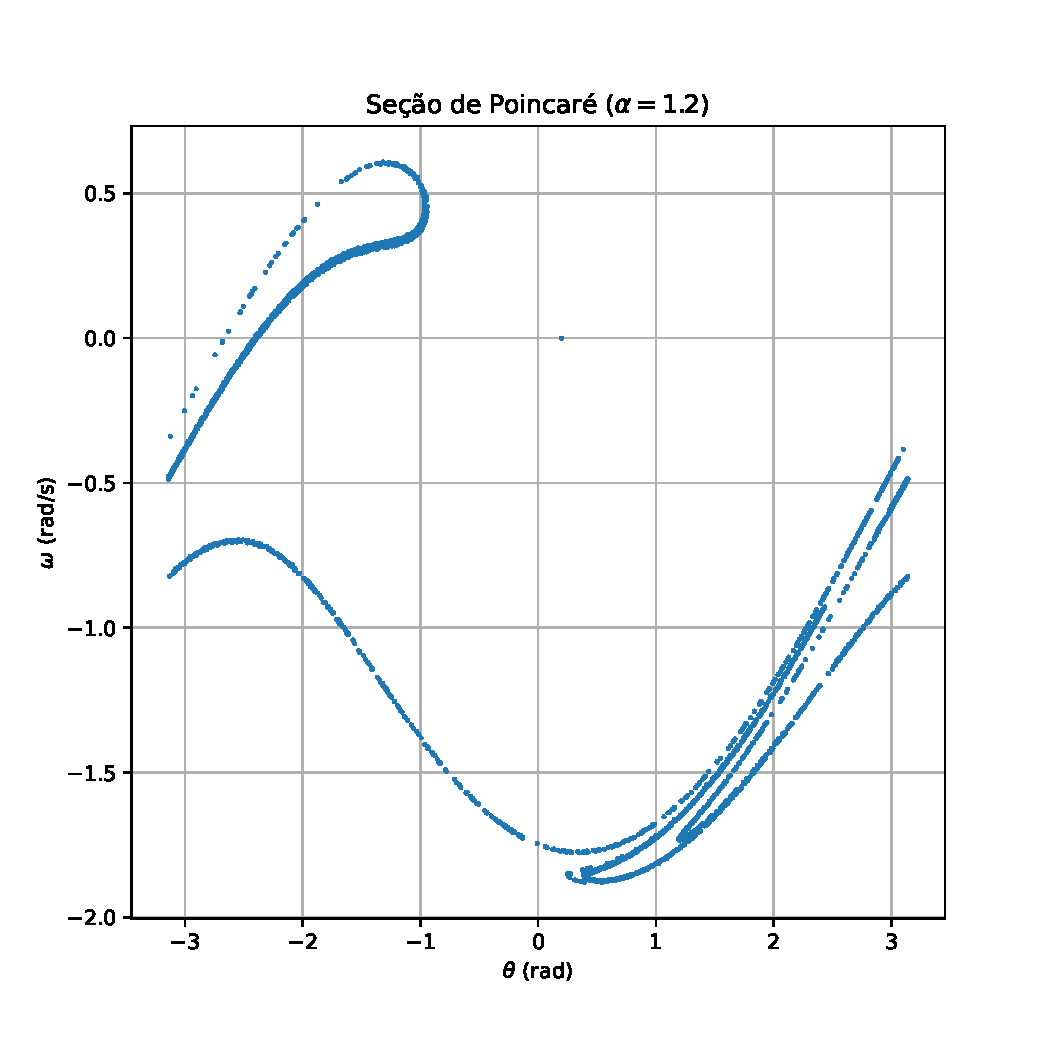
\includegraphics[width=0.4\textwidth]{fig2d2.pdf}
\caption{Seções de Poincaré do pêndulo com \( \Omega_D = \SI{0.55}{\radian\per\second} \) para \( \alpha = \SI{0.5}{\radian\per\second\squared} \) e \( \alpha = \SI{1.2}{\radian\per\second\squared} \).}
\label{fig2d}
\end{figure}

A figura \ref{fig2d} apresenta a seção de Poincaré do pêndulo com \( \Omega_D = \SI{0.55}{\radian\per\second} \) para \( \alpha = \SI{0.5}{\radian\per\second\squared} \) e \( \alpha = \SI{1.2}{\radian\per\second\squared} \).

%\newpage
\subsection{(e)}

Podemos observar que para o caso não-caótico, após o transiente acabar e o sistema oscilar com a frequência \( \Omega_D \), o sistema passa a se encontrar no mesmo estado físico com o mesmo período da força externa.
Também podemos observar que mesmo no caso caótico, ainda existe alguma estrutura previsível, com a formação do atrator estranho.

\newpage
\section{Exercício 3}

\subsection{(a)}

\begin{figure}[ht]
\centering
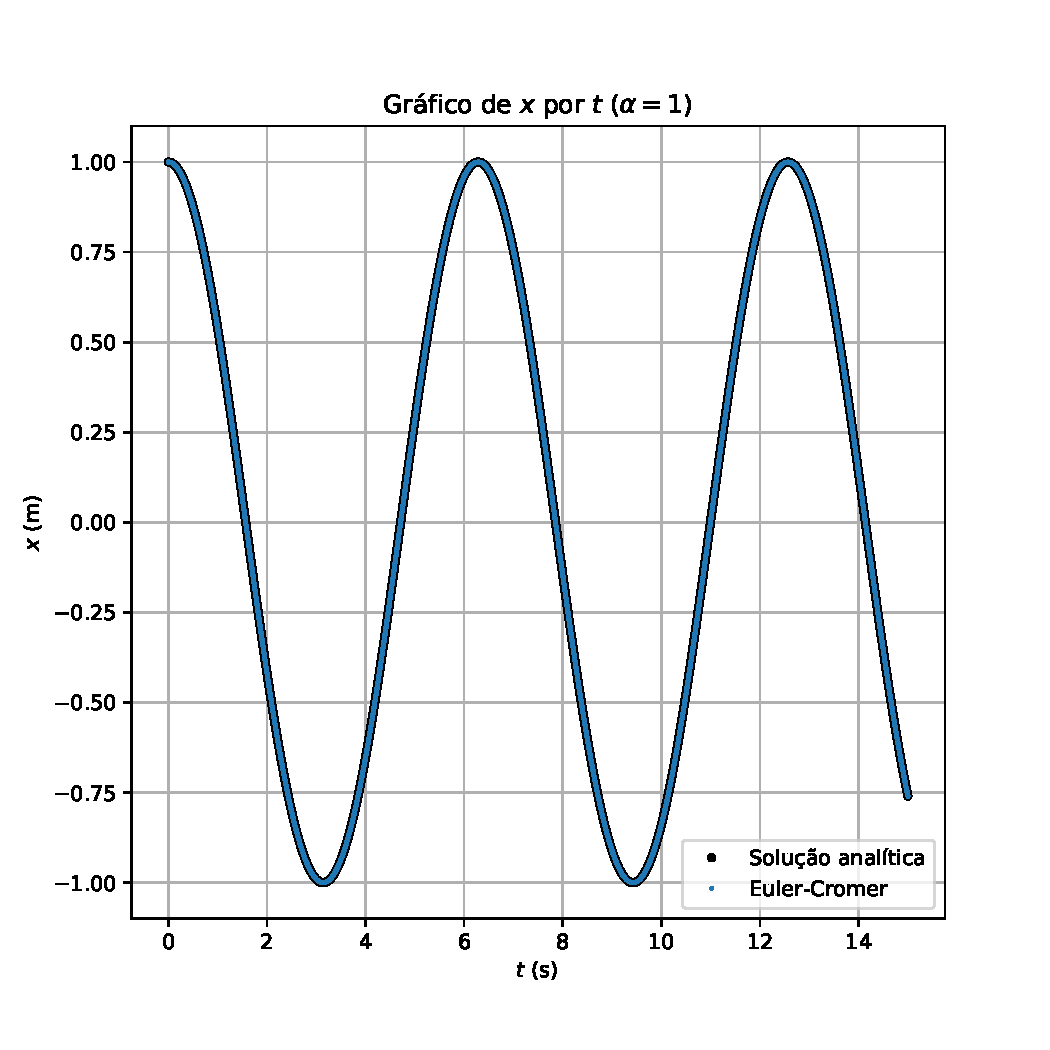
\includegraphics[width=0.7\textwidth]{fig3a.pdf}
\caption{Gráfico de \( x \) por \( t \) para o oscilador com \( \alpha = 1 \).}
\label{fig3a}
\end{figure}

A figura \ref{fig3a} mostra o gráfico da posição em função do tempo para o oscilador no caso \( \alpha = 1 \), que é um oscilador harmônico. Para que a equação de movimento faça sentido, é necessário que a unidade de \( k \) seja
\[ \frac{ \si{\meter\per\second\squared}}{ \si{\meter^\alpha} } = \si{\meter^{1 - \alpha}\per\second\squared} = \si{\newton\per\kilogram\metre^{\alpha}} . \]
O gráfico é idêntico ao do exercício 1, e é mostrada a solução analítica para comparação, que mostra que o método de Euler-Cromer é adequado para esse caso.

\newpage
\subsection{(b)}

\begin{figure}[ht]
\centering
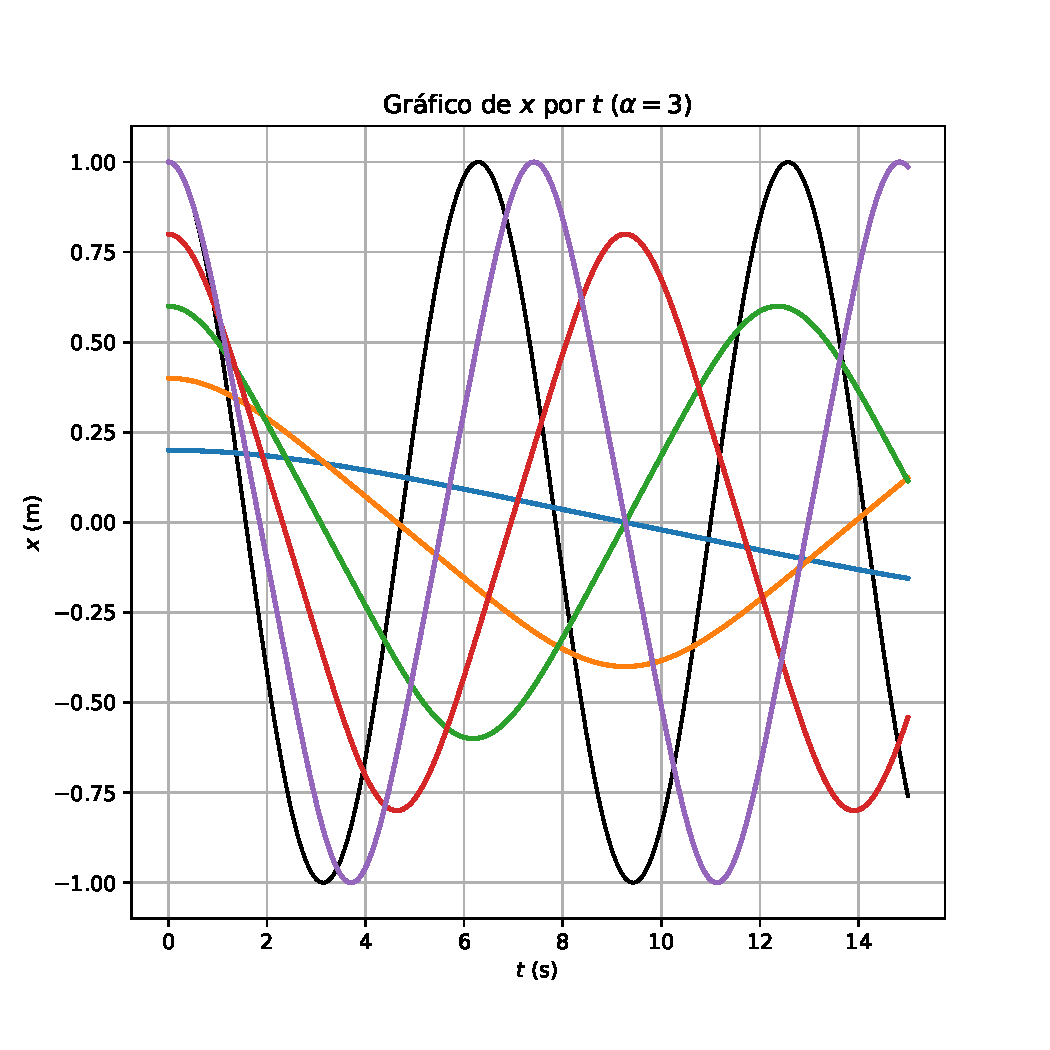
\includegraphics[width=0.7\textwidth]{fig3b.pdf}
\caption{Gráficos de \( x \) por \( t \) para o oscilador com \( \alpha = 3 \) com diferentes condições iniciais e com a solução analítica do caso \( \alpha = 1 \) em preto para comparação.}
\label{fig3b}
\end{figure}

A figura \ref{fig3b} mostra os gráficos da posição em função do tempo para o oscilador no caso \( \alpha = 3 \) com as condições iniciais \( x_0 = \) \SIlist{0.2;0.4;0.6;0.8;1.0}{\metre}.
É possível ver que conforme a amplitude aumenta, o período diminui, diferentemente do caso harmônico.

%\newpage
\subsection{(c)}

Ao comparar o caso \( \alpha = 3 \) com o \( \alpha = 1 \), para distâncias mais próximas da posição de equilíbrio, a força restauradora é muito mais fraca, e para distâncias maiores da posição de equilíbrio, a força restauradora é muito mais intensa.
Isso faz com que o oscilador passe menos tempo nas extremidades e muito mais tempo próximo da posição de equilíbrio do que o caso harmônico, introduzindo a dependência do período com a amplitude.

\end{document}
